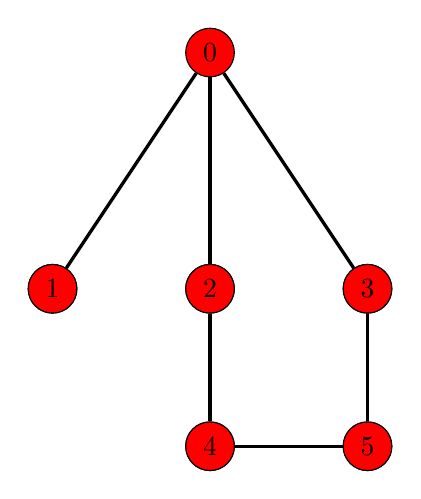
\begin{tikzpicture}
  
  \node[shape=circle,draw=black, fill=red] (0) at (0,0) {0};

  % bfs = [0, 1, 2, 3, 4, 5]

  \node<1>[shape=circle,draw=black] (1) at (-2,-3) {1};
  \node<2->[shape=circle,draw=black,fill=red] (1) at (-2,-3) {1};

  \node<1-2>[shape=circle,draw=black] (2) at (0,-3) {2};
  \node<3->[shape=circle,draw=black, fill=red] (2) at (0,-3) {2};

  \node<1-3>[shape=circle,draw=black] (3) at (2,-3) {3};
  \node<4->[shape=circle,draw=black,fill=red] (3) at (2,-3) {3};

  \node<1-4>[shape=circle,draw=black] (4) at (0,-5) {4};
  \node<5->[shape=circle,draw=black,fill=red] (4) at (0,-5) {4};

  \node<1-5>[shape=circle,draw=black] (5) at (2,-5) {5};
  \node<6->[shape=circle,draw=black,fill=red] (5) at (2,-5) {5};

  \draw[black, very thick] (0) -- (1);
  \draw[black, very thick] (0) -- (2);
  \draw[black, very thick] (0) -- (3);
  \draw[black, very thick] (2) -- (4);
  \draw[black, very thick] (3) -- (5);
  \draw[black, very thick] (4) -- (5);

 \end{tikzpicture}